
\section{Motivation}
\label{sec:motivation}
\bx{This section identifies the research gaps in container-based cloud data center in three resource management processes.}


\bx{Application initial placement is conducted when data centers receive a number of requests for new application deployment.}  The placement can be seen as a static optimization task to allocate applications and reduce energy. 
% The optimization process can be described as: given a number of  PMs represented as resources (e.g CPU cores and RAM etc);  requested applications (wrapped with VMs or container) represented as aforementioned resources; the objective is to allocate these applications into a minimum number of PMs. The decision variable is the location of each application. The basic constraint is that the aggregative resources of hosted VMs cannot exceed the PM's resource capacity.
% The strategies in VM-based cloud and container-based cloud are different. In VM-based cloud, requested applications (wrapped with VMs) are placed into a minimum number of PMs. The problem in VM-based cloud is often modeled as a bin packing problem \cite{Xiong:2014jq}, with VMs represent items and PMs represent bins. The complexity is NP-hard \cite{Hochbaum:1996ts}. 

\bx{In a container-based Cloud, the application initial placement can be seen as a bilevel optimization problem \cite{Colson:2007bu} where each level is bin packing problem.} The lower level optimizes the placement of containers to VMs and the upper level optimizes the placement of VMs to PMs. The advantage the bilevel model is that the interaction of two-level's placement is considered, so that the global optimal can be achieved. Currently, there is no study considers the container-based placement as a bilevel problem.

\bx{Two reasons motivate us to solve the application initial placement in container-based Cloud.} 
First, In order to solve the application intial placement problem, it needs to propose a new bilevel model.
A bilevel model - includes energy model, prices model - is required to represent the relationship between container, VMs, and energy consumption.} Current VM-based models cannot be directly applied because the different problem structure. In addition, current VM-based models normally do not consider the influence of the overhead of VM hypervisor. Furthermore, many previous VM-based models do not consider a balance between resources which is crucial according to previous research \cite{Tomas:2013iv}. 

\bx{Second, we will develop an evolutionary computation (EC)-based approach to solve the bilevel optimization problem.}
Evolutionary computation based algorithms have been proposed to solve bilevel optimization problems \cite{Wang:2008kb, Wang:2011di, Angelo:2013ee} and shown promising performance. On the other hand, traditional algorithms such as Integer linear programming (ILP) has been proposed to solve the bilevel optimization problem, however, it requires a transformation of a bilevel problem into a single-level problem, because the complexity for the bilevel problem is high so that the ILP cannot solve it in a feasible time. 

% The optimization interact with VMs and containers, therefore, it cannot be optimized separately. An additional constraint is that each container has its OS requirement which makes them cannot be simply packed into homogeneous VMs. 

% \bx{Container-based placement can be seen as a bilevel optimization problem \cite{Colson:2007bu} where each level is bin packing problem.} Because of the problem structure has changed, previous VM-based approaches cannot be directly applied on the problem. In addition, currently, there is no study considers the container-based placement as a bilevel problem. The advantage of considering it as a bilevel problem is that containers and VMs can cooperate to achieve lower energy consumption. However, the \emph{optimization of joint placement of container and VMs} is very difficult because of the nature of bilevel problem.

% The hierarchy of bilevel optimization makes problems non-convex and strongly NP-hard \cite{Vicente:1994ie}.
% The placement problem in the VM context has been studied for years \cite{Xu:2010vh, Gao:2013gg, Ferdaus:2014ep} and it is often modeled as a bin packing problem . This is because VMs and PMs are naturally modeled as items and bins. Furthermore, server consolidation and bin-packing have the same optimization objective: minimize the number of bins/PMs. The complexity of bin-packing problem is NP-hard which is NP-hard \cite{Hochbaum:1996ts} which means it is extreme time-consuming to find its optimal solution when the number of decision variables is large. However, most research focus on VM-based server consolidation and these methods cannot be directly applied on container-based consolidation because of the different structure.

% \bx{Only few research focus on container-based server consolidation problem. One of research is from Piraghaj and et al \cite{Piraghaj:2015uf}.} They propose a simple heuristics on two-step allocation, thus, did not consider the interaction between two levels (see detailed discussion in Section \ref{container-based-placement}). 
% In addition, their resource allocation system completely relies on dynamic placement without using static methods. Although their system can execute allocation fast, the energy efficiency cannot be guaranteed. 
% Another research \cite{Mann:2016hx} is the earliest study which realizes two-level of placement should be considered together because they are interact with each other. They apply a fixed VM placement algorithm and considering a series of VM selection algorithms. The results also proves that the interaction between two placement cannot be ignored. 



\vspace{5mm}


% For the lower level of allocation, the objective is to maximize the utilization of resources (e.g a balanced utilization among several resources), while the upper level objective is to minimize the number of PMs. 
\bx{After initial placement, periodic optimization is a routine process that takes existing applications' placement, re-placing them to PMs according to the nature of their workloads (e.g static, periodic or continuously changing etc).} A live migration technique is used to move one application from one PM to another. The live migration is a very expensive operation since it consumes network bandwidth and uses the resource on both host PM and target PM. Therefore, periodic optimization is a multi-objective task which considers minimizing migration of applications and minimizing the overall energy consumption. Resolving the bi-level multi-objective problem will lead to a high utilization of PMs as well as a robust placement of applications.

\bx{Two reasons motivates us to explore solutions for periodic optimization in a container-based cloud}. 
First, periodic optimization in a container-based cloud is a bilevel multi-objective task.
However, so far, there is no research focus on the bilevel multi-objective problem. 
Second, not many research have considered the robustness of placement. To achieve robustness, periodic optimization must consider the variation of workload and plan their positions in advance. This is because workloads' variation may cause overloading or underloading of PMs which requires live migration. However, the major gap in literature is most research simplified workloads as static (remains a constant value throughout its life cycle) \cite{Viswanathan:2012ej, Chen:2011fl,Feller:2011vs} for the sake of simplicity. For example, for periodic work, the average value within a period of time will be considered. 

% \bx{In our research, we will consider periodic optimization as a multi-objective problem with various types of workload \cite{Fehling:2014tl}.} Specifically, complementary workloads can be combined so that it can potentially reduce the migration in the future. Thus, the applications are consolidated in a more robust way. 

% However, in real life, workloads vary with time. According to Fehling , applications' workload are roughly classified into five categories: static, periodic, once-in-a-life-time, continuously changing, and unpredictable. 

% They cannot be treated as a static value in a server consolidation because Therefore, it increases the cost in the future. 




% Only a few research consider applying different strategies on different workloads \cite{Meng:2010gh}. Their experiments showed promising results, however, they only mapped paired workloads which can be further improved by combining multiple workloads.
\vspace{5mm}


\bx{Dynamic placemend is applied on overloading and underloading scenarios which need an immediate reaction \cite{Beloglazov:2013ht}.} In these scenarios, PMs are either running out of resources or running in a low utilization. At these states, applications inside the PM will be placed to other PMs to quickly resolve the problems.
% Overloading is a scenario that the workloads exceed the capacity of its host PM. Hence, one or more applications will be migrated to other PMs. Underloading is when a PM runs in a low utilization, all the applications inside it will be moved to other PMs, so that the PM can be turned off. The common operation in these two scenarios are the dynamic placement \cite{Xiao:2015ik}. Dynamic placement places one application each time in an on-line manner. 

\bx{Two reasons for us to solve dynamic placement.} 
First, we want to develop a uniform algorithm to solve the dynamic placment with various workloads. Current dynamic placement approaches typically applied either simple bin-packing algorithms such as First Fit or manually design heuristics. Simple bin-packing algorithms may perform poorly because application placement is more complicated than bin-packing \cite{Mann:2015ua}, while manual designed heuristics may not be general because they are designed for specific conditions and constraints\cite{Jung:2010dt}. Therefore, we will consider using hyper-heuristic approach such as genetic programming to automatically generate heuristics. 
% The hyper-heuristic can learn from previous good solutions as well as the features of various workloads so that the dispatching rules can be applied with any conditions and constraints. 
% on one hand, dynamic placement allocates an application at a time to meet the requirement of fast reaction. On the other hand, it only considers the best placement of the current application using either simple bin-packing algorithms such as First Fit or manually design heuristics. Simple bin-packing algorithms may perform poorly because application placement is more complicated than bin-packing \cite{Mann:2015ua}, while manual designed heuristics may not be general because they are designed for specific conditions and constraints\cite{Jung:2010dt}.
% Mann's research  showed, server consolidation is a lot harder than bin-packing problem because of the multi-dimensional of resources, heterogeneous PMs, migration cost etc. 

\bx{Second, we want to develop an approach which achieves both fast and global optimization on dynamic placement problem.}
However, since the applications are placed one at each time, it is difficult to achieve fast placement and global optimization at the same time.
% \bx{These challenges motivate us to develop a hyper-heuristic approach which can automatically generate heuristics for quickly placing.} 

% In addition, in container-based Cloud, the placement target is on containers and the destination is a suitable VM. However, if no VM can accommodate a container, a new VM must be created, which incurs a second level of deployment.

% \bx{In summary, this thesis aims at improving the energy efficiency in a container-based cloud data center.} The gaps in three resource management processes motivate us to address three issues:
% \begin{itemize}
% 	\item Develop an algorithm for the joint placement of containers and VMs.
% 	\item Develop an algorithm for multi-objective joint placement of containers and VMs with consider various workloads.
% 	\item Develop a hyper-heuristic for dynamic placement.
% \end{itemize}




% The motivation for this thesis mainly includes two parts, in the first part, we illustrate the roots of container-based server consolidation problem. In the second parts, we explain the motivations for the objectives.

% \subsection{Motivation For Container-based Server Consolidation Problem}

% Server consolidation \cite{Zhang:2010vo} resolves the low utilization problem by gathering applications or VMs into a fewer number of physical machines (PMs), so that the resource utilization of PMs are maintained at a high level. In the meanwhile, idle servers are turned off to save energy. Traditional server consolidation is VM-based, in comparison with 
% a server host a single application, it can dramatically improve the resource utilization. 


% \begin{figure}
% 	\centering
% 	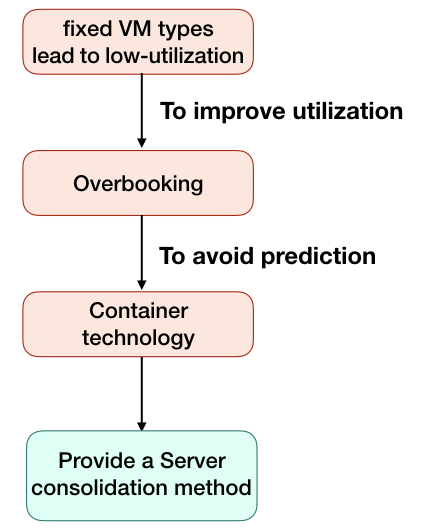
\includegraphics[width=0.3\textwidth]{pics/problem_flow.png}
% 	\caption{The root of container technology}
% 	\label{fig:root}
% \end{figure}
% \begin{enumerate}
% \item Container is a new virtualization technology which provides an operating level of virtualization.
% % Figure \ref{fig:root} illustrates the root of container technology from an energy efficient point of view. 

% In order to solve this problem, overbooking strategy tends to place more VMs than the server's maximum capacity. However, this technique is highly relied on workload prediction on the application running in a VM. Otherwise, servers are easily overloaded. Container technique can improve the utilization by further partitioning VM into resource isolated chunks. Therefore, multiple applications can share the same VM. This technique avoids the prediction of workload as well as improving the utilization. 



% This container technology brings many advantages to current Cloud industry\cite{Felter:2015ki}but it also brings difficulties for server consolidation. Container-based server consolidation adds another level of abstraction which makes it a two-level vector bin-packing problem.
% Therefore, it motivates us to provide \emph{global optimized} resource allocation solution for container-based data centers.

% \end{enumerate}


% \subsection{Motivation For Research objectives}
% Cloud data center has a high dynamic nature where it constrantly receives new requests for resource provisioning and releases old current resources. Therefore, a data center needs different strategies to
% handle different scenarios. 

% \textcolor{Maroon}{In this thesis, we aim at providing a series of approaches to continuously optimize the joint allocation of VMs and containers which involves with three scenarios: application initial placement, periodic consolidation, and dynamic consolidation.} Different stages have distinct goals, therefore, they are considered as separated research questions. 

% \begin{enumerate}
% \item Joint allocation of containers and VMs (application initial placement), \\
% \textcolor{Maroon}{Joint allocation of containers and VMs is the first task when a data center receives new application deployment requests.} At this stage, a set of containers is allocated to a set of VMs and these VMs are allocated to a set of PMs. This task is challenging because the problem is a bilevel optimization where each level is a bin packing problem. Exhaustive search of entire solution space is practically impossible, for the number of possible permutation of solution is huge. Current approaches \cite{Piraghaj:2016bw,Hindman:2011ux} use simple heuristics such as First Fit to solve the problem. These greedy-based heuristics do not consider the complex structure of the problem, therefore, often reach a local optimal solution.

% Only a few research focus on this  problem, Piraghaj \cite{Piraghaj:2016bw} designs a dynamic allocation system. She proposes a two-step procedure. Since, these two-level structure interact each other, separate solution certainly leads to a local optima. Therefore, in this thesis, we will solve the problem simutaneously.
% Most importantly, and therefore can not be solved separately. This is the first research that consider server consolidation has a bi-level optimization problem \cite{Wen:1991kt}. 

% In this objective, we will establish the fundamental concepts in studying this joint allocation of containers and VMs including new problem models: price and power model, new problem constraints, and optimization objectives. The major challenges for this objective is to design representations and several EC approaches to solve this problem. More specifically, in designing the EC approach, new search mechanisms, operators will be designed and new representations will be proposed to fit the problem. 

% This task is challenging, since a representation can highly affect the performance of consolidation \cite{SoteloFigueroa:2013be}. 

% \item Periodic consolidation, \\
% \textcolor{Maroon}{A periodic consolidation is conducted to improve the global energy efficiency in a periodical fashion.} Data center constantly receives new allocations, releasing of old resources. These changing degrades the compact structure of a data center. Therefore, the data center needs a global optimization to improve the overall energy efficiency.

% The challenges are three folds, firstly, similar with initialization problem, the problem has two level of allocations and they interact with each other. Secondly, like VM-based consolidation, Container-based consolidation is considered as a multi-objective problem with minimization of migration cost as well as keeping a good energy efficiency. In bilevel optimization, multi-objective can be defined in either or both level, therefore, it further increases the complexity. Thirdly, consolidation needs to consider different types of workload which may lead to more migrations in the future(\textcolor{Maroon}{NEED MORE EXPLANATION}).

% \item Dynamic consolidation,\\
% Dynamic It takes one container and allocates it to VMs. Since the size of container can be dynamically adjusted, when the an application is under-provision or over-provision, the original container is halted, resized and re-allocated. Hence, there is a need to allocate this new container in real time.

% To solve a dynamic consolidation, heuristics and dispatching rules are often used \cite{Sarin:2011fu, Shi:2011ke, Forsman:2015ca, Beloglazov:2012ji}.  In this scenario, a dispatching rule is considered as a function that determines the priorities of VMs that a container can be placed. However, dynamic placement is much complex than bin-packing problem \cite{Mann:2015ua}. Because of its dynamic nature, human designed heuristics are ill-equipped in approximating solutions when the environment has changed \cite{SoteloFigueroa:2013be}. 

% Hyper-heuristic methods, sepcifically, Genetic Programming (GP) technique \cite{Banzhaf:1998wc} can learn from the best previous allocation and automatically evolves dispatching rules to solve this problem. GP has been applied in generating dispatching rules for bin-packing problem \cite{Burke:2006ei, SoteloFigueroa:2013be} and other scheduling problems \cite{Nguyen:2014eu}. The results have shown promising results.

% There are mainly two challenges, first, it is difficult to identify the related factors that construct the heuristic. Factors or features are the building blocks of heuristics. It is a difficult task because the relationship between a good heuristic and features are not obvious. Second, representations provide different patterns to construct dispatching rules. It is also unclear what representation is the most suitable for the consolidation problem.


% and representations must be proposed to capture the characteristic of the joint allocation. 
% 	and the VMs are allocated to physical machines in the second step. Because of the complexity, previous research
% 	only considers the first step. They map the incoming tasks into predefined categories and based on the characteristic of the categories, the size of new virtual machines' resources are decided. After each tasks have chosen its VM type, they are allocated to virtual machines using a lightweight heursitic algorithm. 
% 	We intend to apply an EC-based approach to solve this problem by proposing a coevolutionary that simuetiously decide the virtual machine type as well as the allocation of VMs.


% \item Large-scale of static server consolidation problem, \\
	% In this case, initialization and periodic consolidation are belonged to this category. 
	% Since Cloud data center typically has hundreds of thousands PMs and more, static server consolidation is always very challenging. Many approaches have been proposed in the literature to resolve the problem. There are mainly two ways, both relied on distributed methods, hierarchical-based \cite{Jung:2010dt, Moens:2011gk} and agent-based management systems \cite{Yazir:2010bk}.
	% The major problem in agent-based systems is that agents rely on heavy communication to maintain a high-level utilization. Therefore, it causes heavy load in the networking. 
	% Hierarchical-based approaches are the predominate methods. In essence, these approaches are centralized methods where all the states of PMs within its region are collected and analyzed. The major disadvantage of hierarchical-based approaches is that it only provides local solutions. In fact, it is infeasible and unnecessary to check all the states of PMs since the search space is too large and most PMs do not need a change. This idea
	% motivates a way to improving the effectiveness is to reduce the number of variables so that the search space is narrowed. In this thesis, we are going to investigate the way to eliminate the redundant information.
% \end{enumerate}



% Traditional Cloud computing offers three services models: Infrastructure as a Service (IaaS), Platform as a Service (PaaS) and Software as a Service (SaaS). Both IaaS and PaaS describe how does a service provider use the cloud resources. The main difference of these two models are  
% IaaS allows service providers to manage the low-level details including the operating system and libraries. While, PaaS provides a higher level of abstraction where users only focus on the application development without caring the underlying operating system and system-level of resources such as CPU cores and memories. However, one drawback of PaaS is that cloud users must make sure their applications are complete compatible with the platform. And in many of the cases, it is not the situation. In order to solve this problem, a container-based virtualization technology starts to reform the Cloud industry. Container as a Service (CaaS) 
% is a new concept but it has been used in industry for many years. Containers provide an operating system-level of isolation environment for applications. It does not need a hypervisor but complete rely on the operating system. 


% This exciting new technology has bring so many advantages for both Cloud users and Cloud providers. From the providers' perspective, In a large system, running VMs means there are probably many same operating systems occupying memories and storages. Lightweight containers share operating system and therefore, there are more rooms for softwares. It increases the capability of Cloud data centers. Furthermore, in terms of resource utilization, it provides much finer granularity operation than a VM-based Cloud model. Containers partition
% a VM into smaller chunks so that with appropriate management, better energy efficiency can be achieved. From the cloud users' perspective, each container provides separated libraries for specific application.  Therefore, it does not contrained by the underlying platform. Like PaaS, Cloud users do not need to concern the scalability of applications. 
% Therefore, CaaS can potentially become one of the main stream in the future Cloud computing industry. 

% Secondly, energy-efficent computing has been the major concern since the begining of computers. Specifially, Cloud computing has become a popular form. Large-scale data centers have been built around the world. A data center can consume huge amount of energies and it needs to improve its energy-efficiency from multiple perspectives. As we discussed in the Introduction, computing servers are one of the major contribution to the energy consumption. 
% And according to observation by \cite{}, the average utilization resource are still very low which causes huge energy wastage. As we mentioned above, the container technolgy provides a better way of managing resources, it has the potential to largly improve the utilization than current VM-based Cloud model because it avoids some of the major drawbacks of VM-based model. 

% Thirdly, because the container technology is relatively new, previous research are mostly focus on IaaS model and so that the server consolidation has based on the VM-level. However,   

% Frist is this new technology of container that can potentially change the landscape of
% Cloud computing. It has so many benefits but also it brings difficulty in managing resources.

% Second, from green computing point of view, we still need to manage resource so that, the 
% data centers consume less energy. And container technolgy actually bring a better chance to
% be more energy-efficient than previous VM based technology.
% Third, it is very difficult to manage this container-based resources because of the problem-nature is too complicated. And existed algorithms can not be directly applied on it.
% Fourth, the evolutioanry computation provides a good framework to handle such difficult problem.

% \textcolor{Blue}{Motivation is what is now lack from the literature.} \\

% The advantage of Platform as a Service (PaaS) has been discovered in the recent years. 
% The disadvantage of tranditional IaaS model has been discovered in the recent years \cite{Mann:2016hx}.
% In IaaS, on one hand, cloud customers need to manage the low-level details ranging from application capacity estimation,
% resource planning and selection and deployment. 
% On the other hand, Cloud providers manage resource provisioning and allocation. 
% Although these two tasks are seemingly different, 


% The container as a Service (CaaS) cloud model has gain increasing attention in the recent years.
% However, the energy efficiency in CaaS cloud environment has not been investigate. 
% Particularly, the virtual machine and container joint consolidation is the core problem.
% Therefore, in this thesis, we will focus on the end-to-end energy-aware server consolidation on container-based
% Cloud. In the meanwhile,  a major research direction of large scale server consolidation is also considered. 
% The end-to-end server consolidation refers to the server consolidation techniques used
% in the different stages throughout the routine Cloud resource management including  initial VM provisioning and placement, dynamic VM placement, and static VM placement:
